\documentclass{extbook}[14pt]
\usepackage{multicol, enumerate, enumitem, hyperref, color, soul, setspace, parskip, fancyhdr, amssymb, amsthm, amsmath, bbm, latexsym, units, mathtools}
\everymath{\displaystyle}
\usepackage[headsep=0.5cm,headheight=0cm, left=1 in,right= 1 in,top= 1 in,bottom= 1 in]{geometry}
\usepackage{dashrule}  % Package to use the command below to create lines between items
\newcommand{\litem}[1]{\item #1

\rule{\textwidth}{0.4pt}}
\pagestyle{fancy}
\lhead{}
\chead{Answer Key for Makeup Progress Quiz -1 Version A}
\rhead{}
\lfoot{7547-2949}
\cfoot{}
\rfoot{Fall 2020}
\begin{document}
\textbf{This key should allow you to understand why you choose the option you did (beyond just getting a question right or wrong). \href{https://xronos.clas.ufl.edu/mac1105spring2020/courseDescriptionAndMisc/Exams/LearningFromResults}{More instructions on how to use this key can be found here}.}

\textbf{If you have a suggestion to make the keys better, \href{https://forms.gle/CZkbZmPbC9XALEE88}{please fill out the short survey here}.}

\textit{Note: This key is auto-generated and may contain issues and/or errors. The keys are reviewed after each exam to ensure grading is done accurately. If there are issues (like duplicate options), they are noted in the offline gradebook. The keys are a work-in-progress to give students as many resources to improve as possible.}

\rule{\textwidth}{0.4pt}

\begin{enumerate}\litem{
Solve the rational equation below. Then, choose the interval(s) that the solution(s) belongs to.
\[ \frac{-6}{7x -3} + -4 = \frac{2}{-42x + 18} \]

The solution is \( x = 0.226 \), which is option C.\begin{enumerate}[label=\Alph*.]
\item \( x \in [-0.67,-0.6] \)

$x = -0.631$, which corresponds to not distributing the factor $7x -3$ correctly when trying to eliminate the fraction.
\item \( x_1 \in [0.08, 0.22] \text{ and } x_2 \in [-0.77,1.23] \)

$x = 0.143 \text{ and } x = 0.226$, which corresponds to getting the correct solution and believing there should be a second solution to the equation.
\item \( x \in [0.23,1.23] \)

* $x = 0.226$, which is the correct option.
\item \( \text{All solutions lead to invalid or complex values in the equation.} \)

This corresponds to thinking $x = 0.226$ leads to dividing by zero in the original equation, which it does not.
\item \( x_1 \in [-0.67, -0.6] \text{ and } x_2 \in [-0.77,1.23] \)

$x = -0.631 \text{ and } x = 0.226$, which corresponds to getting the correct solution and believing there should be a second solution to the equation.
\end{enumerate}

\textbf{General Comment:} Distractors are different based on the number of solutions. Remember that after solving, we need to make sure our solution does not make the original equation divide by zero!
}
\litem{
Choose the graph of the equation below.
\[ f(x) = \frac{-1}{(x - 2)^2} - 2 \]

The solution is the graph below, which is option E.
\begin{center}
    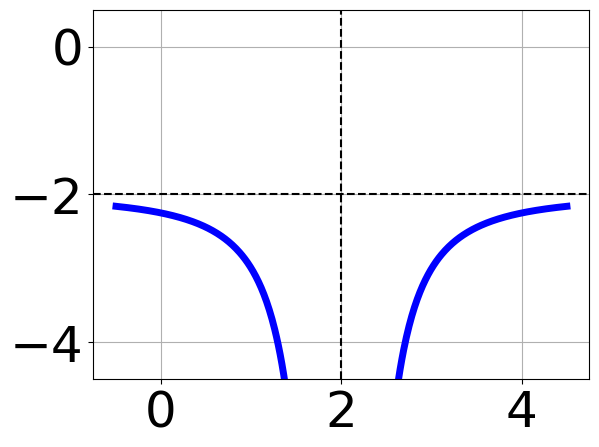
\includegraphics[width=0.3\textwidth]{../Figures/rationalEquationToGraphCopyEA.png}
\end{center}\begin{enumerate}[label=\Alph*.]
\begin{multicols}{2}
\item 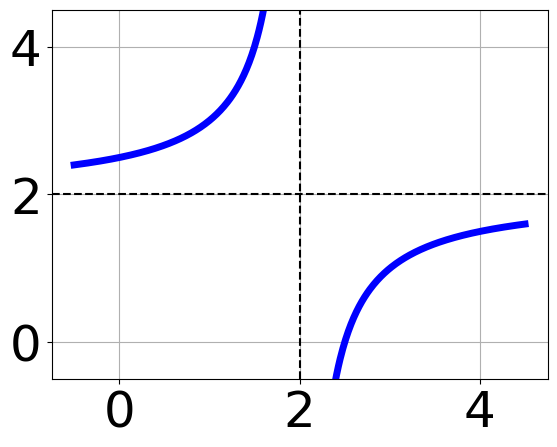
\includegraphics[width = 0.3\textwidth]{../Figures/rationalEquationToGraphCopyAA.png}
\item 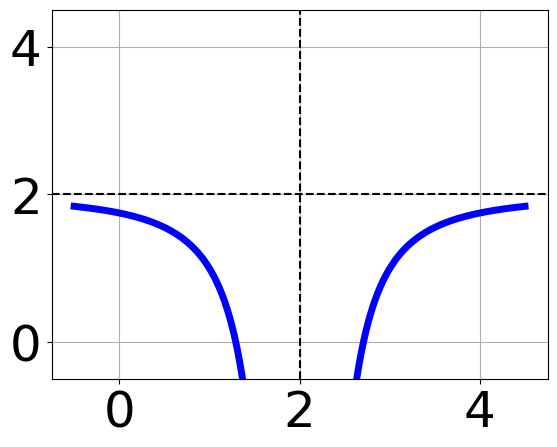
\includegraphics[width = 0.3\textwidth]{../Figures/rationalEquationToGraphCopyBA.png}
\item 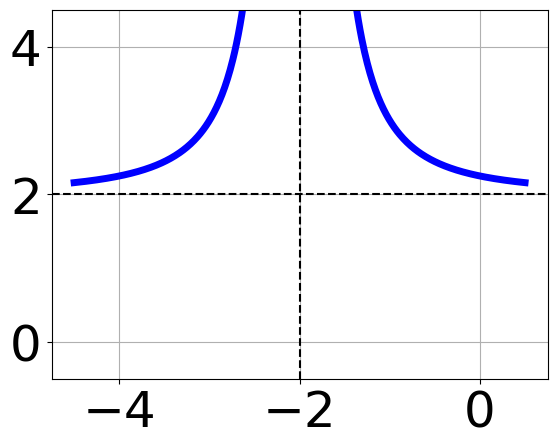
\includegraphics[width = 0.3\textwidth]{../Figures/rationalEquationToGraphCopyCA.png}
\item 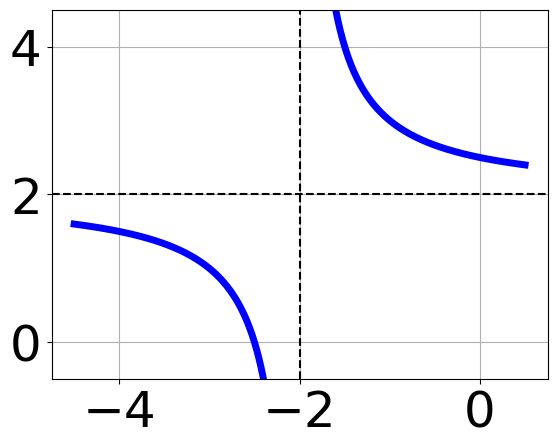
\includegraphics[width = 0.3\textwidth]{../Figures/rationalEquationToGraphCopyDA.png}
\end{multicols}\item None of the above.\end{enumerate}
\textbf{General Comment:} Remember that the general form of a basic rational equation is $ f(x) = \frac{a}{(x-h)^n} + k$, where $a$ is the leading coefficient (and in this case, we assume is either $1$ or $-1$), $n$ is the degree (in this case, either $1$ or $2$), and $(h, k)$ is the intersection of the asymptotes.
}
\litem{
Solve the rational equation below. Then, choose the interval(s) that the solution(s) belongs to.
\[ \frac{98}{-112x + 112} + 1 = \frac{98}{-112x + 112} \]

The solution is \( \text{all solutions are invalid or lead to complex values in the equation.} \), which is option D.\begin{enumerate}[label=\Alph*.]
\item \( x_1 \in [-4, 0] \text{ and } x_2 \in [1,2] \)

$x = -1.000 \text{ and } x = 1.000$, which corresponds to getting the correct solution and believing there should be a second solution to the equation.
\item \( x \in [-4,0] \)

$x = -1.000$, which corresponds to not distributing the factor $-112x + 112$ correctly when trying to eliminate the fraction.
\item \( x_1 \in [0, 4] \text{ and } x_2 \in [1,2] \)

$x = 1.000 \text{ and } x = 1.000$, which corresponds to getting the correct solution and believing there should be a second solution to the equation.
\item \( \text{All solutions lead to invalid or complex values in the equation.} \)

*$x = 1.000$ leads to dividing by 0 in the original equation and thus is not a valid solution, which is the correct option.
\item \( x \in [1.0,2.0] \)

$x = 1.000$, which corresponds to not checking if this value leads to dividing by 0 in the original equation and thus is not a valid solution.
\end{enumerate}

\textbf{General Comment:} Distractors are different based on the number of solutions. Remember that after solving, we need to make sure our solution does not make the original equation divide by zero!
}
\litem{
Determine the domain of the function below.
\[ f(x) = \frac{3}{15x^{2} -24 x + 9} \]

The solution is \( \text{All Real numbers except } x = 0.600 \text{ and } x = 1.000. \), which is option D.\begin{enumerate}[label=\Alph*.]
\item \( \text{All Real numbers except } x = a, \text{ where } a \in [0.44, 0.71] \)

All Real numbers except $x = 0.600$, which corresponds to removing only 1 value from the denominator.
\item \( \text{All Real numbers.} \)

This corresponds to thinking the denominator has complex roots or that rational functions have a domain of all Real numbers.
\item \( \text{All Real numbers except } x = a \text{ and } x = b, \text{ where } a \in [8.87, 9.33] \text{ and } b \in [14.87, 15.1] \)

All Real numbers except $x = 9.000$ and $x = 15.000$, which corresponds to not factoring the denominator correctly.
\item \( \text{All Real numbers except } x = a \text{ and } x = b, \text{ where } a \in [0.44, 0.71] \text{ and } b \in [0.8, 1.45] \)

All Real numbers except $x = 0.600$ and $x = 1.000$, which is the correct option.
\item \( \text{All Real numbers except } x = a, \text{ where } a \in [8.87, 9.33] \)

All Real numbers except $x = 9.000$, which corresponds to removing a distractor value from the denominator.
\end{enumerate}

\textbf{General Comment:} Recall that dividing by zero is not a real number. Therefore the domain is all real numbers \textbf{except} those that make the denominator 0.
}
\litem{
Choose the equation of the function graphed below.

\begin{center}
    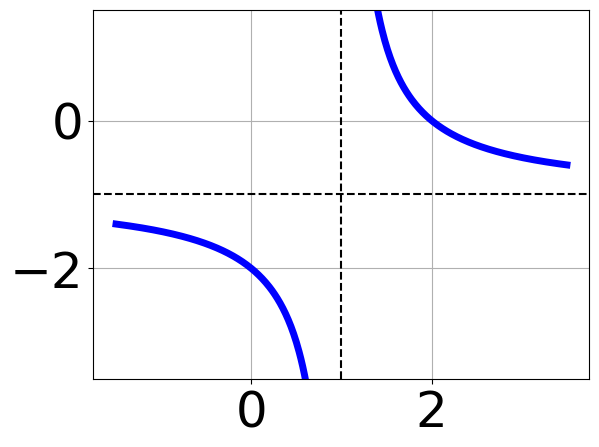
\includegraphics[width=0.5\textwidth]{../Figures/rationalGraphToEquationCopyA.png}
\end{center}




The solution is \( \text{None of the above as it should be } f(x) = \frac{1}{x - 1} - 1 \), which is option E.\begin{enumerate}[label=\Alph*.]
\item \( f(x) = \frac{-1}{x - 1} + 3 \)

Corresponds to using the general form $f(x) = \frac{a}{x-h}+k$, the opposite leading coefficient AND not noticing the $y$-value was wrong.
\item \( f(x) = \frac{1}{(x + 1)^2} + 3 \)

Corresponds to thinking the graph was a shifted version of $\frac{1}{x^2}$ not noticing the $y$-value was wrong.
\item \( f(x) = \frac{-1}{(x - 1)^2} + 3 \)

Corresponds to thinking the graph was a shifted version of $\frac{1}{x^2}$, using the general form $f(x) = \frac{a}{x-h}+k$, the opposite leading coefficient, AND not noticing the $y$-value was wrong.
\item \( f(x) = \frac{1}{x + 1} + 3 \)

The $x$- and $y$-value of the equation does not match the graph.
\item \( \text{None of the above} \)

None of the equation options were the correct equation.
\end{enumerate}

\textbf{General Comment:} Remember that the general form of a basic rational equation is $ f(x) = \frac{a}{(x-h)^n} + k$, where $a$ is the leading coefficient (and in this case, we assume is either $1$ or $-1$), $n$ is the degree (in this case, either $1$ or $2$), and $(h, k)$ is the intersection of the asymptotes.
}
\litem{
Determine the domain of the function below.
\[ f(x) = \frac{3}{30x^{2} -6 x -36} \]

The solution is \( \text{All Real numbers except } x = -1.000 \text{ and } x = 1.200. \), which is option E.\begin{enumerate}[label=\Alph*.]
\item \( \text{All Real numbers.} \)

This corresponds to thinking the denominator has complex roots or that rational functions have a domain of all Real numbers.
\item \( \text{All Real numbers except } x = a, \text{ where } a \in [-37, -29] \)

All Real numbers except $x = -36.000$, which corresponds to removing a distractor value from the denominator.
\item \( \text{All Real numbers except } x = a, \text{ where } a \in [-2, 0] \)

All Real numbers except $x = -1.000$, which corresponds to removing only 1 value from the denominator.
\item \( \text{All Real numbers except } x = a \text{ and } x = b, \text{ where } a \in [-37, -29] \text{ and } b \in [29, 31] \)

All Real numbers except $x = -36.000$ and $x = 30.000$, which corresponds to not factoring the denominator correctly.
\item \( \text{All Real numbers except } x = a \text{ and } x = b, \text{ where } a \in [-2, 0] \text{ and } b \in [-0.8, 5.2] \)

All Real numbers except $x = -1.000$ and $x = 1.200$, which is the correct option.
\end{enumerate}

\textbf{General Comment:} Recall that dividing by zero is not a real number. Therefore the domain is all real numbers \textbf{except} those that make the denominator 0.
}
\litem{
Choose the equation of the function graphed below.

\begin{center}
    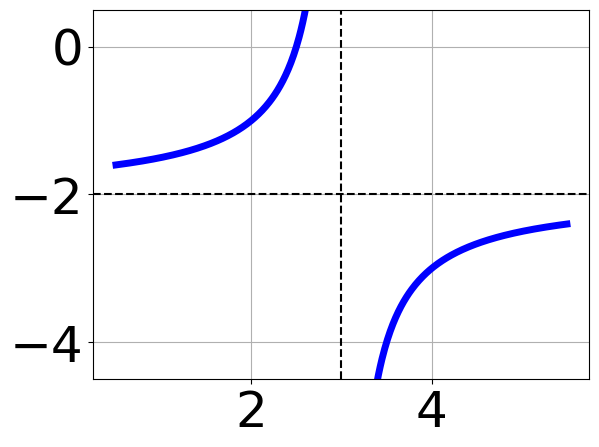
\includegraphics[width=0.5\textwidth]{../Figures/rationalGraphToEquationA.png}
\end{center}




The solution is \( \text{None of the above as it should be } f(x) = \frac{-1}{x - 3} - 2 \), which is option E.\begin{enumerate}[label=\Alph*.]
\item \( f(x) = \frac{1}{x - 3} - 4 \)

Corresponds to using the general form $f(x) = \frac{a}{x-h}+k$, the opposite leading coefficient AND not noticing the $y$-value was wrong.
\item \( f(x) = \frac{1}{(x - 3)^2} - 4 \)

Corresponds to thinking the graph was a shifted version of $\frac{1}{x^2}$, using the general form $f(x) = \frac{a}{x-h}+k$, the opposite leading coefficient, AND not noticing the $y$-value was wrong.
\item \( f(x) = \frac{-1}{(x + 3)^2} - 4 \)

Corresponds to thinking the graph was a shifted version of $\frac{1}{x^2}$ not noticing the $y$-value was wrong.
\item \( f(x) = \frac{-1}{x + 3} - 4 \)

The $x$- and $y$-value of the equation does not match the graph.
\item \( \text{None of the above} \)

None of the equation options were the correct equation.
\end{enumerate}

\textbf{General Comment:} Remember that the general form of a basic rational equation is $ f(x) = \frac{a}{(x-h)^n} + k$, where $a$ is the leading coefficient (and in this case, we assume is either $1$ or $-1$), $n$ is the degree (in this case, either $1$ or $2$), and $(h, k)$ is the intersection of the asymptotes.
}
\litem{
Solve the rational equation below. Then, choose the interval(s) that the solution(s) belongs to.
\[ \frac{-7x}{-7x + 2} + \frac{-6x^{2}}{28x^{2} -43 x + 10} = \frac{3}{-4x + 5} \]

The solution is \( \text{There are two solutions: } x = -0.293 \text{ and } x = 0.930 \), which is option D.\begin{enumerate}[label=\Alph*.]
\item \( x \in [1.03,2.15] \)


\item \( \text{All solutions lead to invalid or complex values in the equation.} \)


\item \( x_1 \in [-1.12, 0.7] \text{ and } x_2 \in [-0.32,0.42] \)


\item \( x_1 \in [-1.12, 0.7] \text{ and } x_2 \in [0.87,1.03] \)

* $x = -0.293 \text{ and } x = 0.930$, which is the correct option.
\item \( x \in [-0.17,1.08] \)


\end{enumerate}

\textbf{General Comment:} Distractors are different based on the number of solutions. Remember that after solving, we need to make sure our solution does not make the original equation divide by zero!
}
\litem{
Choose the graph of the equation below.
\[ f(x) = \frac{1}{x + 1} + 3 \]

The solution is the graph below, which is option E.
\begin{center}
    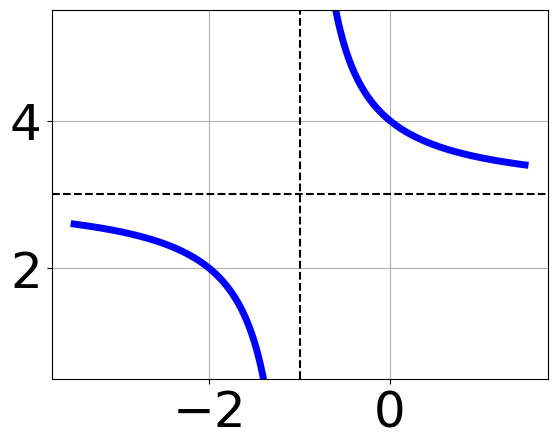
\includegraphics[width=0.3\textwidth]{../Figures/rationalEquationToGraphEA.png}
\end{center}\begin{enumerate}[label=\Alph*.]
\begin{multicols}{2}
\item 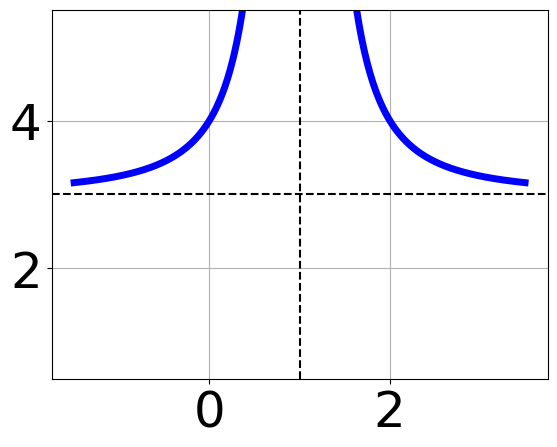
\includegraphics[width = 0.3\textwidth]{../Figures/rationalEquationToGraphAA.png}
\item 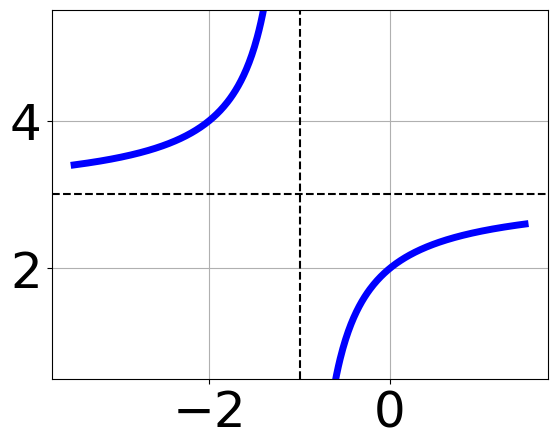
\includegraphics[width = 0.3\textwidth]{../Figures/rationalEquationToGraphBA.png}
\item 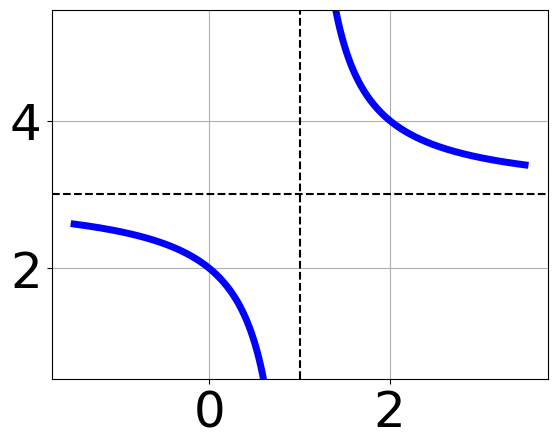
\includegraphics[width = 0.3\textwidth]{../Figures/rationalEquationToGraphCA.png}
\item 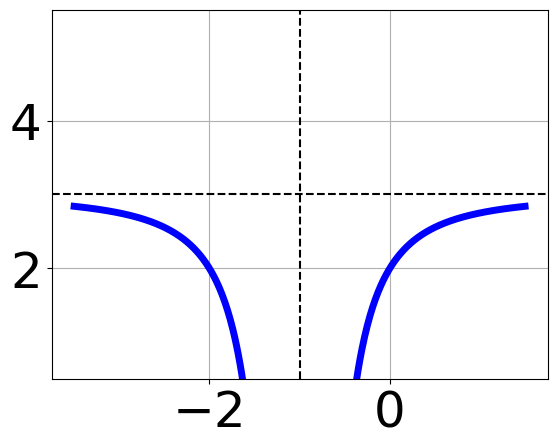
\includegraphics[width = 0.3\textwidth]{../Figures/rationalEquationToGraphDA.png}
\end{multicols}\item None of the above.\end{enumerate}
\textbf{General Comment:} Remember that the general form of a basic rational equation is $ f(x) = \frac{a}{(x-h)^n} + k$, where $a$ is the leading coefficient (and in this case, we assume is either $1$ or $-1$), $n$ is the degree (in this case, either $1$ or $2$), and $(h, k)$ is the intersection of the asymptotes.
}
\litem{
Solve the rational equation below. Then, choose the interval(s) that the solution(s) belongs to.
\[ \frac{6x}{7x + 2} + \frac{-7x^{2}}{-42x^{2} +2 x + 4} = \frac{-3}{-6x + 2} \]

The solution is \( \text{There are two solutions: } x = -0.152 \text{ and } x = 0.919 \), which is option E.\begin{enumerate}[label=\Alph*.]
\item \( \text{All solutions lead to invalid or complex values in the equation.} \)


\item \( x_1 \in [-0.76, 0.14] \text{ and } x_2 \in [-1.12,0.47] \)


\item \( x \in [0.53,1.03] \)


\item \( x \in [0.3,0.48] \)


\item \( x_1 \in [-0.76, 0.14] \text{ and } x_2 \in [0.74,3.18] \)

* $x = -0.152 \text{ and } x = 0.919$, which is the correct option.
\end{enumerate}

\textbf{General Comment:} Distractors are different based on the number of solutions. Remember that after solving, we need to make sure our solution does not make the original equation divide by zero!
}
\end{enumerate}

\end{document}